\section{Nested optimization details}

\subsection{Search and registry}
For outer scenario $q$, the other nine scenarios are split into three deterministic inner groups. The staged search evaluates representation before sparse sensing, recovery on fixed placement anchors, placement with frozen recovery, and a bounded joint recheck. The resulting files contain \OptValidationRecords{} sparse train-validation rows, \OptOuterRecords{} outer rows and \OptPlacementRecords{} prespecified outer placement-audit rows. Configurations, scenario identifiers, objective values, solver settings and seeds are stored per row; no failed configuration is omitted (none failed in the completed run).

The two final independent-property representations use spatial ranks $(80,48)$ or $(64,48)$ for each property and 16 modal coefficients per property. Scaling is no transform in most folds and RMS scaling in the remainder. Property weights in these independent models algebraically cancel between the per-property fit and expansion and are not interpreted as a source of gain. The joint tensor comparator uses $(80,48,2,32)$ with min--max scaling in every fold.

\subsection{Recovery and placement}
Recovery candidates are minimum-norm LS, relative ridge, L1 ADMM and elastic net. The selected family varies by fold and budget; the complete frozen mapping is in \path{selected_sparse_strategies.json}. Condition-aware, determinant-greedy, configured, whitened-QR, cluster-constrained and well-region placements are all retained in \path{outer_placement_audit.csv}. Random placement uses 20 deterministic orders per fold and is collapsed to one fold median before statistical summaries.

Pressure-objective well order is more stable than joint order (mean Kendall $\tau=\OptWellRankTau$ for condition-aware pressure ranking). The corrected cluster experiment uses active cells only and selects $k$ from train-only silhouette and adjusted-Rand stability. It chooses $k=5$ in every outer-training fit, but does not improve the 30-channel outer benchmark; it becomes competitive only at larger grid budgets.

\subsection{Statistics and reproducibility}
Every table reports ten outer-fold values through mean/standard deviation and median/interquartile summaries. Paired Wilcoxon tests are descriptive because the folds share one fixed-geology ensemble. The generated file \path{paired_statistics.csv} includes raw and Holm-adjusted values; the conservative adjustment covers all comparisons in each metric family, so no broad superiority claim is based on an isolated raw value.

The independent reproduction refits the accuracy TBMD, compression TBMD and POD-E for all outer folds using only frozen JSON selections. All 2,160 identity/configuration records match. Reconstruction metrics agree within absolute tolerance $10^{-10}$ (observed maximum below $3\times10^{-14}$); condition numbers agree within relative tolerance $10^{-12}$. Runtime is excluded from exact equality because it is hardware- and load-dependent.

\subsubsection{Detailed optimization results}


\subsubsection{Representation bottlenecks and train-selected architecture}
The nested study confirms that the original TBMD gap is principally a spatial-truncation floor rather than an unavoidable consequence of tensor representation. At fixed modal depth, inner-validation pressure error falls sharply when $R_2$ reaches the full second grid dimension and continues to improve with $R_1$ (Fig.~\ref{fig:opt_rank}). The original basis has outer full-state pressure/saturation RMSE \OptRepOriginalPressure/\OptRepOriginalSaturation; the train-selected joint $(80,48,2,32)$ basis reaches \OptRepJointPressure/\OptRepJointSaturation. Independent property heads give the lowest equal-property normalized objective, \OptRepAccuracyJoint, while POD-E remains better for pressure alone (\OptRepPodePressure{} versus \OptRepAccuracyPressure). The accuracy and compression TBMD bases store \OptAccuracyCompression{} and \OptCompressionCompression{} times fewer values than rank-32 POD-E (Fig.~\ref{fig:opt_compression}).

\begin{figure}[tbp]
\centering
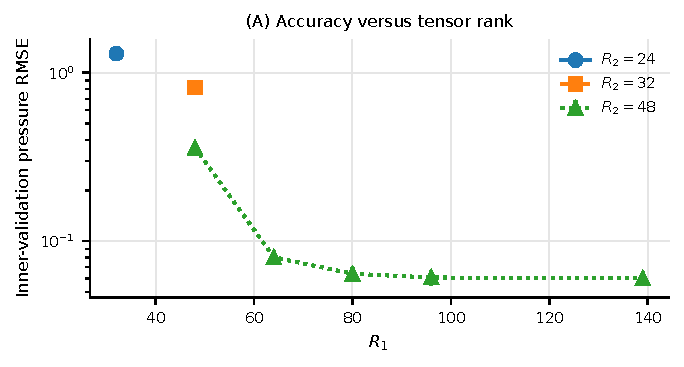
\includegraphics[width=0.62\textwidth]{../../../../studies/brugge_sparse_sensing/figures/fig8_rank_accuracy.pdf}
\caption{Inner-validation pressure RMSE versus spatial tensor ranks at modal rank 16. Error bars show variation across the 30 outer/inner training partitions. The low-$R_2$ configurations are retained as failed accuracy regimes rather than removed from the registry.}
\label{fig:opt_rank}
\end{figure}

\begin{figure}[tbp]
\centering
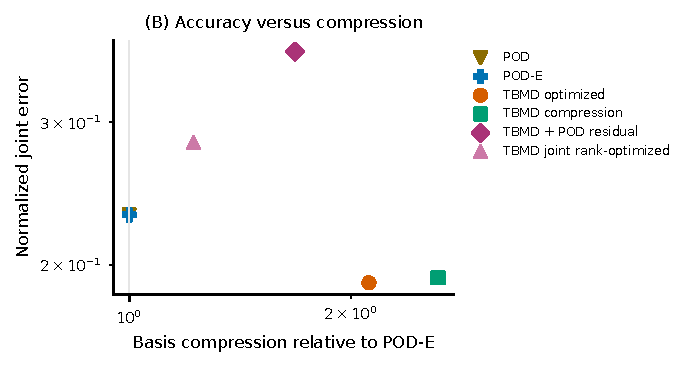
\includegraphics[width=\textwidth]{../../../../studies/brugge_sparse_sensing/figures/fig9_accuracy_compression.pdf}
\caption{Untouched outer full-state normalized joint error versus basis-storage compression relative to POD-E. Pressure and saturation errors are reported separately in the generated tables; the scalar objective does not replace them.}
\label{fig:opt_compression}
\end{figure}

\begin{table*}[t]
\centering
\caption{Evolution of TBMD. Validation gain is relative reduction of the train-only representation objective from the original basis; outer errors use 30 joint wells.}
\label{tab:tbmd_evolution}
\footnotesize
\setlength{\tabcolsep}{2.5pt}
\begin{tabular}{@{}p{0.20\linewidth}p{0.27\linewidth}rrrr@{}}
\toprule
TBMD version & Key change & \shortstack{Validation\\gain} & \shortstack{Pressure\\RMSE ($u_p$)} & \shortstack{$S_o$\\RMSE} & \shortstack{Stored\\floats} \\
\midrule
Original TBMD & Fixed HOOI ranks (48,48,2), fixed L1 & 0.0\% & 0.4323 & 0.004251 & 101.9k \\
Original basis + optimized sensing & Nested placement/recovery & 0.0\% & 0.4289 & 0.004235 & 101.9k \\
Rank-optimized joint TBMD & Spatial/modal rank expansion & 89.8\% & 0.0892 & 0.000643 & 259.2k \\
TBMD + residual & Low-rank POD residual & 86.8\% & 0.2117 & 0.000788 & 188.7k \\
Compressed independent TBMD & Independent properties; 5\% validation tolerance & 93.1\% & 0.1754 & 0.000651 & 120.7k \\
Accuracy-selected independent TBMD & Independent properties; minimum validation loss & 93.2\% & 0.1787 & 0.000644 & 149.7k \\
\bottomrule
\end{tabular}
\end{table*}


\subsubsection{Sparse reconstruction and conditioning}
With joint measurements from all existing wells, POD-E remains the strongest comparator: pressure RMSE is $\OptWellThirtyPodePressure\pm\OptWellThirtyPodePressureSd$, compared with \OptWellThirtyJointPressure{} for rank-optimized joint TBMD and \OptWellThirtyCompressionPressure{} for the compressed independent model (Table~1 of the main manuscript). The original basis remains poor after nested recovery and placement optimization, so recovery alone cannot remove its representation floor. Median budget curves (Fig.~\ref{fig:opt_budget}) also show that placement/regularization transitions can produce non-monotone error; no monotonicity is assumed.

Independent property heads are difficult to observe from joint wells: their block basis has median condition numbers several orders of magnitude above POD-E over much of the budget range (Fig.~\ref{fig:opt_condition}). Ridge, L1 and elastic-net selection controls the resulting variance but does not make conditioning irrelevant. Conversely, pressure-only fitting favours TBMD for pressure (\OptPressureWellThirtyCompressionPressure{} versus \OptPressureWellThirtyPodePressure{} at 30 wells), while its independent saturation head is unobserved. That result is not a joint-state reconstruction advantage.

\begin{figure}[tbp]
\centering
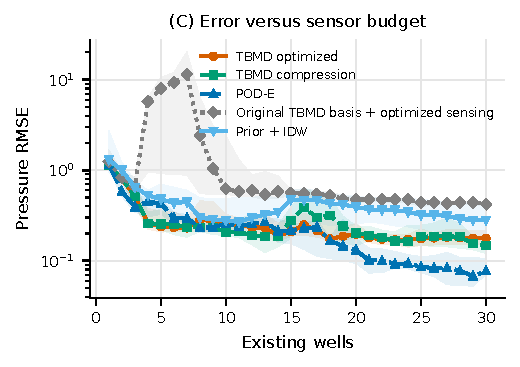
\includegraphics[width=0.62\textwidth]{../../../../studies/brugge_sparse_sensing/figures/fig10_sensor_budget.pdf}
\caption{Median pressure RMSE and interquartile band across outer folds versus the number of existing joint-property wells. Every curve uses parameters selected inside its outer-training partition.}
\label{fig:opt_budget}
\end{figure}

\begin{figure}[tbp]
\centering
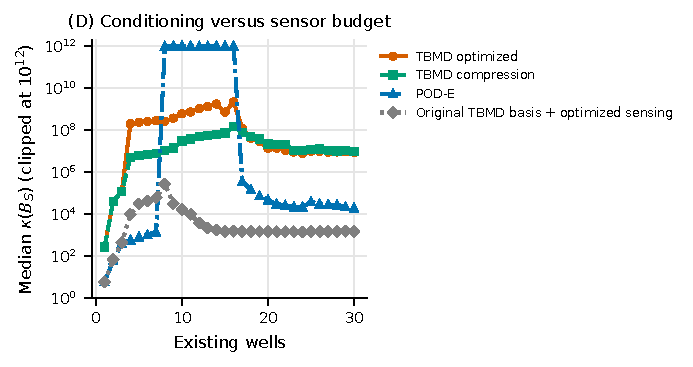
\includegraphics[width=\textwidth]{../../../../studies/brugge_sparse_sensing/figures/fig11_conditioning.pdf}
\caption{Median condition number of the sampled basis versus existing-well budget. Values above $10^{12}$ are clipped only for plotting and remain unmodified in the canonical CSV output.}
\label{fig:opt_condition}
\end{figure}

All-well results are reported in Table~1 of the main manuscript.

\subsubsection{Regime-specific advantage and Pareto decision}
At 100 grid channels, optimized independent TBMD lowers the normalized joint error to \OptGridHundredAccuracyJoint{} from POD-E's \OptGridHundredPodeJoint; at 300 channels the compressed model reaches \OptGridThreeHundredCompressionJoint{} versus \OptGridThreeHundredPodeJoint. The tensor model has higher pressure error but lower saturation error; at 300 channels its joint objective is lower in all ten folds. This identifies a dense-grid, saturation-aware regime rather than universal TBMD superiority.

The ablation (Fig.~\ref{fig:opt_ablation}) attributes the largest gain to correcting tensor ranks. Property separation improves full-state and high-grid-budget joint accuracy, but rank-optimized joint TBMD is better at existing joint wells; the POD-residual hybrid does not supply a consistent additional gain. The Pareto map (the Pareto figure in the main manuscript) therefore supports a regime-specific conclusion: POD-E is preferred for existing joint wells and pressure accuracy, while optimized TBMD occupies the accuracy--storage frontier and can improve the equal-property objective when sufficiently many grid channels observe both properties.

\begin{figure}[tbp]
\centering
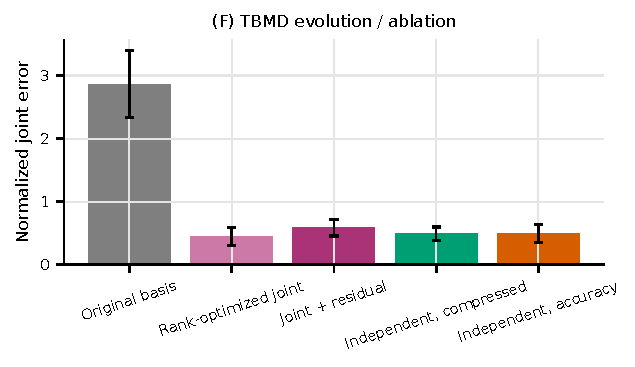
\includegraphics[width=0.68\textwidth]{../../../../studies/brugge_sparse_sensing/figures/fig13_ablation.pdf}
\caption{TBMD evolution/ablation at all 30 joint wells. Bars show mean normalized joint error and error bars show one standard deviation across outer folds.}
\label{fig:opt_ablation}
\end{figure}



\subsubsection{Well ranking and corrected clustering}
Pressure-objective well rankings are stable across folds (mean pairwise Kendall $\tau=\OptWellRankTau$). Early-ranked wells concentrate in regions of higher pressure variability (Fig.~\ref{fig:opt_wells}), but this association is descriptive and does not establish geological causality. The corrected clustering uses active cells only, deterministic seeds, and train-selected silhouette/stability criteria. It selects five clusters in every outer-training fit, but performs poorly at 30 channels and is only competitive at larger budgets. Clustering is therefore retained in the Supplement and registry, not promoted as a main method.

\begin{figure}[tbp]
\centering
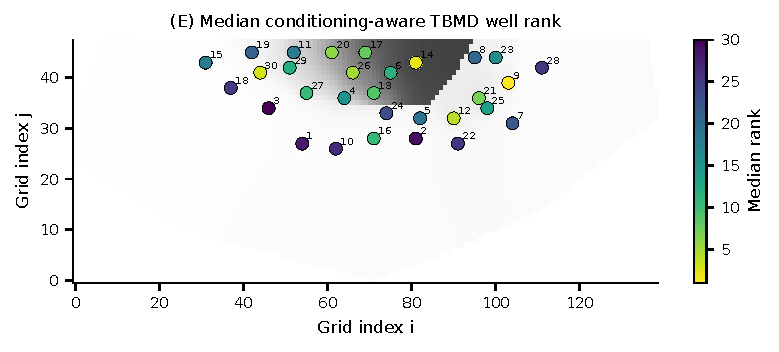
\includegraphics[width=\textwidth]{../../../../studies/brugge_sparse_sensing/figures/fig12_well_ranking.pdf}
\caption{Median conditioning-aware rank of the 30 existing wells for optimized TBMD. Labels are the configured well indices; lower ranks are selected earlier. The background is pressure variability over the supplied ensemble.}
\label{fig:opt_wells}
\end{figure}

\begin{table*}[t]
\centering
\caption{Untouched leave-one-scenario-out reconstruction from all 30 existing wells, with the no-measurement prior shown at zero wells. Values are mean $\pm$ standard deviation across ten outer folds. Bold entries are selected automatically as the smallest column mean.}
\label{tab:optimization_diagnostics}
\resizebox{\textwidth}{!}{%
\begin{tabular}{lrrrrrr}
\toprule
Method & Wells & Pressure RMSE & $S_o$ RMSE & Compression & Storage & Online ms \\
\midrule
POD-E random & 30 & \textbf{0.0840 $\pm$ 0.0273} & \textbf{0.000575 $\pm$ 0.000130} & 1.00$\times$ & 316.8k & -- \\
POD-E & 30 & \textbf{0.0840 $\pm$ 0.0273} & \textbf{0.000575 $\pm$ 0.000130} & 1.00$\times$ & 316.8k & 0.596 \\
TBMD joint rank-optimized & 30 & 0.0892 $\pm$ 0.0234 & 0.000643 $\pm$ 0.000132 & 1.22$\times$ & 259.2k & 1.447 \\
TBMD compression & 30 & 0.1754 $\pm$ 0.0835 & 0.000651 $\pm$ 0.000118 & 2.62$\times$ & 120.7k & 1.476 \\
TBMD optimized & 30 & 0.1787 $\pm$ 0.0463 & 0.000644 $\pm$ 0.000129 & 2.12$\times$ & 149.7k & 1.196 \\
POD & 30 & 0.2164 $\pm$ 0.1231 & 0.000756 $\pm$ 0.000258 & 1.00$\times$ & 316.8k & 0.001 \\
Prior + IDW & 30 & 0.3127 $\pm$ 0.1647 & 0.000780 $\pm$ 0.000197 & -- & 0.0k & -- \\
Original TBMD + tuning & 30 & 0.4289 $\pm$ 0.0506 & 0.004235 $\pm$ 0.000027 & 3.11$\times$ & 101.9k & 0.132 \\
Prior & 0 & 1.1481 $\pm$ 0.5580 & 0.000839 $\pm$ 0.000213 & -- & 0.0k & 0.000 \\
\bottomrule
\end{tabular}
}
\end{table*}

